\documentclass[12pt]{article}

\usepackage[margin=1in]{geometry}
\usepackage{amsmath, amssymb, amsthm}
\usepackage{graphicx}
\usepackage{booktabs}
\usepackage{hyperref}
\usepackage{natbib}
\usepackage{setspace}
\usepackage{caption}
\usepackage{float}
\usepackage{xeCJK}
\usepackage{fontspec}

\setCJKmainfont{FandolSong-Regular}
\setCJKsansfont{FandolHei-Regular}

\onehalfspacing

\title{魔法少女、公共品与进化稳定：\\
一个基于《魔法少女小圆》的偏好演化模型}
\author{}
\date{}

\begin{document}

\maketitle

\begin{center}
    \textbf{Abstract / 抽象}
\end{center}


\noindent
本文将动画《魔法少女小圆》中三位核心角色——佐仓杏子、巴麻美与美树沙耶香——分别映射为经济学中三种偏好类型：纯自利型（homo oeconomicus）、纯康德型（homo kantiensis）与纯利他型（pure altruist），并在凹型公共品博弈框架下分析其战略选择与进化命运。借助 Alger \& Weibull（2013）提出的同类匹配（assortative matching）机制和标准复制动态，模拟结果揭示：沙耶香的纯利他偏好在进化上始终处于劣势；杏子与麻美之间的“胜负”则由匹配同类率 $\sigma$ 决定——低 $\sigma$ 时搭便车占优，高 $\sigma$ 时康德型主导。


%-----------------------------------------------------------------------
\section{引言}
%-----------------------------------------------------------------------

《魔法少女小圆》并非一部关于正义必胜的故事，而是一部关于\textbf{偏好如何决定命运}的寓言。三位主角的行动逻辑各异：杏子从不为他人牺牲自身利益；麻美以"对所有人都正确的选择"为行动准则；沙耶香则将他人的幸福置于自身之上，不计代价。

这三种逻辑恰好对应经济学中三种经典偏好类型，并可在进化博弈论框架下进行严格分析。本文的核心问题是：\textbf{在一个魔女持续侵扰、魔法少女不断死亡与诞生的世界里，哪种偏好类型在进化上能够存活？}

值得指出的是，旧系统的设计者丘比并非传统意义上的反派：它代表的是一种极端的\textbf{宇宙功利主义}——少女在希望与绝望间的情感落差能够产生能量，用于对抗宇宙热寂，因此个体的牺牲在宇宙尺度的成本收益计算下变得"合理"。这与 Alger \& Weibull（2013）的理论框架形成了直接对位：后者证明，当个体之间存在足够的同类接触（高 $\sigma$）时，进化会自然选出带有道德权重的偏好，而不是丘比式的聚合效用最大化。换言之，$\sigma = 0$ 的极端——所有人匿名相遇、个体完全可替换——正是丘比系统的数学对应；而高 $\sigma$ 的共同体，则是其对立面。

%-----------------------------------------------------------------------
\section{模型设定}
%-----------------------------------------------------------------------

\subsection{博弈：凹型公共品博弈}

\textbf{博弈}（game）描述的是这样一种情境：多个参与者各自做出决策，而每个人的结果不仅取决于自己的选择，也取决于他人的选择。在本模型中，每次互动由两位魔法少女参与，每人选择一个\textbf{策略}——即向公共战斗中投入多少资源，用 $x \in [0,1]$ 表示（0 为完全不出力，1 为倾尽全力）。双方都能从对方的贡献中受益（因为共同消灭了更多魔女，带来悲叹之种），但贡献本身需要消耗个人资源，存在自我牺牲的代价。这构成了一个\textbf{社会困境}：对集体最优的选择（双方都积极贡献）与对个人最优的选择（搭便车，让对方多出力）之间存在冲突。

两人之间进行如下\textbf{凹型公共品博弈}（Concave Public Goods Game）：
\begin{equation}
    \pi(x_i, x_j) = r(x_i + x_j) - \frac{r(x_i + x_j)^2}{2} - x_i,
    \label{eq:pgg}
\end{equation}
其中参数 $r = 3$（公共品回报率，$r > 1$ 以保证合作有社会价值），$x_i \in [0,1]$ 为个体 $i$ 的贡献量，$x_i + x_j$ 为双方总贡献，$-r(x_i+x_j)^2/2$ 为拥挤效应（边际回报递减），$-x_i$ 为贡献的个人成本。

与线性公共品博弈不同，该博弈具有\textbf{凹型回报结构}：总贡献越高，边际公共品收益越低。这使得"最优贡献量"存在一个有限的内点解，而非角点解，从而天然地将三种类型的均衡策略区分开来。

社会困境依然存在：每个人都有搭便车的动机（多出一单位贡献，个人成本为 1，但收益 $r - r(x_i+x_j)$ 随总贡献增大而下降）。

\subsection{角色与偏好类型}

每个角色在决策时最大化自己的\textbf{效用函数}（utility function）——即她真正在意的目标。效用函数未必等于物质收益：纯自利者在意自己赚到多少，纯康德型在意"若所有人都这样做"的结果，纯利他者在意对方赚到多少。三种类型的效用函数各不相同，因此即使面对同样的博弈，她们会选择不同的贡献量。

在此博弈框架下，三位角色被映射为如下偏好类型（表~\ref{tab:types}）。各类型均衡策略的完整推导见第~\ref{sub:equilibrium}~节。

\begin{table}[H]
    \centering
    \caption{角色与偏好类型}
    \label{tab:types}
    \begin{tabular}{llll}
        \toprule
        角色 & 偏好类型 & 效用函数 & 均衡策略 \\
        \midrule
        佐仓杏子 & 纯自利（Homo Oeconomicus） & $u_K = \pi(x, y)$ & $x_K^* = \dfrac{r-1}{2r}$ \\[8pt]
        巴麻美   & 纯康德型（Homo Kantiensis） & $u_M = \pi(x, x)$ & $x_M^* = \dfrac{2r-1}{4r}$ \\[8pt]
        美树沙耶香 & 纯利他型（Pure Altruist）  & $u_S = \pi(y, x)$ & $x_S^* = \dfrac{1}{2}$ \\
        \bottomrule
    \end{tabular}
\end{table}

其中 $x \in [0,1]$ 为贡献策略，$\pi(x_i, x_j)$ 为式~\eqref{eq:pgg} 所定义的个体 $i$ 的物质收益。

\paragraph{杏子（纯自利）} 最大化自身物质收益 $\pi(x,y)$。在对手策略给定时，她选择对自己最有利的贡献量，本质上是纳什均衡策略。她不考虑道德，也不关心他人——这与原作中杏子"只为自己而战"的人设完全吻合。

\paragraph{麻美（纯康德型）} 遵循康德式道德律令：选择使"若所有人都如此行动"时收益最大的策略，即最大化 $\pi(x,x)$。值得注意的是，这一策略恰好等于社会计划者的最优解——麻美的康德动机在此博弈中与社会利益完全一致。

\paragraph{沙耶香（纯利他型）} 最大化\textbf{对手}的物质收益 $\pi(y,x)$，即选择令对方收益最高的贡献量，完全不计自身损失。这一设定呼应原作中沙耶香"为了他人不惜一切"的行动逻辑，以及她最终因过度自我牺牲而走向悲剧的结局。

\subsection{均衡策略的推导}\label{sub:equilibrium}

\textbf{均衡策略}（equilibrium strategy）指的是：给定对手的策略，自己无法通过改变贡献量来提高效用——即各类型在自身效用函数下的最优选择。需要注意的是，三种类型的"均衡"性质略有差异：杏子最大化的是物质收益 $\pi$，其均衡是经典意义上的\textbf{纳什均衡}（Nash Equilibrium，双方互为最优反应）；而麻美和沙耶香最大化的效用函数与 $\pi$ 不同，其均衡更准确地称为\textbf{类型特定均衡策略}（type-specific equilibrium strategy）——各自在自身偏好下的最优解，而非针对物质收益的纳什均衡。求解方法在形式上相同：对各自的效用函数关于 $x$ 求导并令导数为零（\textbf{一阶条件}），再代入对称条件 $x = y$（双方同类型时出相同策略）。这一对称条件反映了一个重要的信息假设：\textbf{每种类型的均衡策略是在"假设对手与自己同类型"的前提下推导得出的}，而非基于种群中各类型的实际比例 $\{s_j\}$。各类型的 $x_i^*$ 对种群构成一无所知——种群份额 $s_j$ 仅出现在适应度公式~\eqref{eq:fitness} 中，用于汇总不同类型配对下的期望物质收益，不进入任何个体的最优化问题。

对 \eqref{eq:pgg} 分别对 $x$ 求偏导，令各类型的效用函数一阶条件为零：

\paragraph{杏子}
杏子最大化自身物质收益，将 $\pi(x_i, x_j)$ 中第一个参数代入 $x$、第二个代入 $y$：
$$u_K = \pi(x,y) = r(x+y) - \frac{r(x+y)^2}{2} - x.$$
对 $x$ 求导：
$$\frac{\partial u_K}{\partial x} = r - r(x+y) - 1 = 0 \implies x + y = \frac{r-1}{r}.$$
注意末尾的 $-1$，它来自成本项 $-x$ 的导数，代表杏子承担的边际贡献成本。对称纳什均衡（$x = y$）：$x_K^* = \dfrac{r-1}{2r} = \dfrac{1}{3}$（$r=3$时）。

\paragraph{麻美}
麻美最大化"若所有人都出 $x$"时的收益，即令两个参数相同：
$$u_M = \pi(x,x) = r(2x) - \frac{r(2x)^2}{2} - x = 2rx - 2rx^2 - x.$$
对 $x$ 求导：
$$\frac{\partial u_M}{\partial x} = 2r - 4rx - 1 = 0 \implies x_M^* = \frac{2r-1}{4r} = \frac{5}{12} \approx 0.417.$$
此即\textbf{社会最优解}：令总福利 $2\pi(x,x)$ 最大的 $x$。麻美的康德偏好恰好实现了社会计划者的目标。

\paragraph{沙耶香}
沙耶香最大化对手的物质收益，即令 $\pi$ 的第一个参数为对手策略 $y$、第二个为自己的策略 $x$：
$$u_S = \pi(y,x) = r(y+x) - \frac{r(y+x)^2}{2} - y.$$
注意成本项是 $-y$（对手的成本），而非 $-x$。对 $x$ 求导时，$-y$ 的导数为零：
$$\frac{\partial u_S}{\partial x} = r - r(y+x) = 0 \implies x = 1 - y.$$
这里没有 $-1$，正因为沙耶香的贡献成本 $-x$ 根本不出现在她的效用函数里。对称均衡（$x = y$）：$x_S^* = \dfrac{1}{2}$（与 $r$ 无关）。

三者的大小关系对任意 $r > 1$ 均成立：
\begin{equation}
    x_K^* \;=\; \frac{r-1}{2r} \;<\; x_M^* \;=\; \frac{2r-1}{4r} \;<\; x_S^* \;=\; \frac{1}{2}.
\end{equation}
沙耶香的贡献量超过社会最优 $x_M^*$，意味着她在帮助他人的同时，承担了超过边际社会价值的额外成本。

图~\ref{fig:strategies} 直观展示了三者的目标函数及均衡点。

\begin{figure}[H]
    \centering
    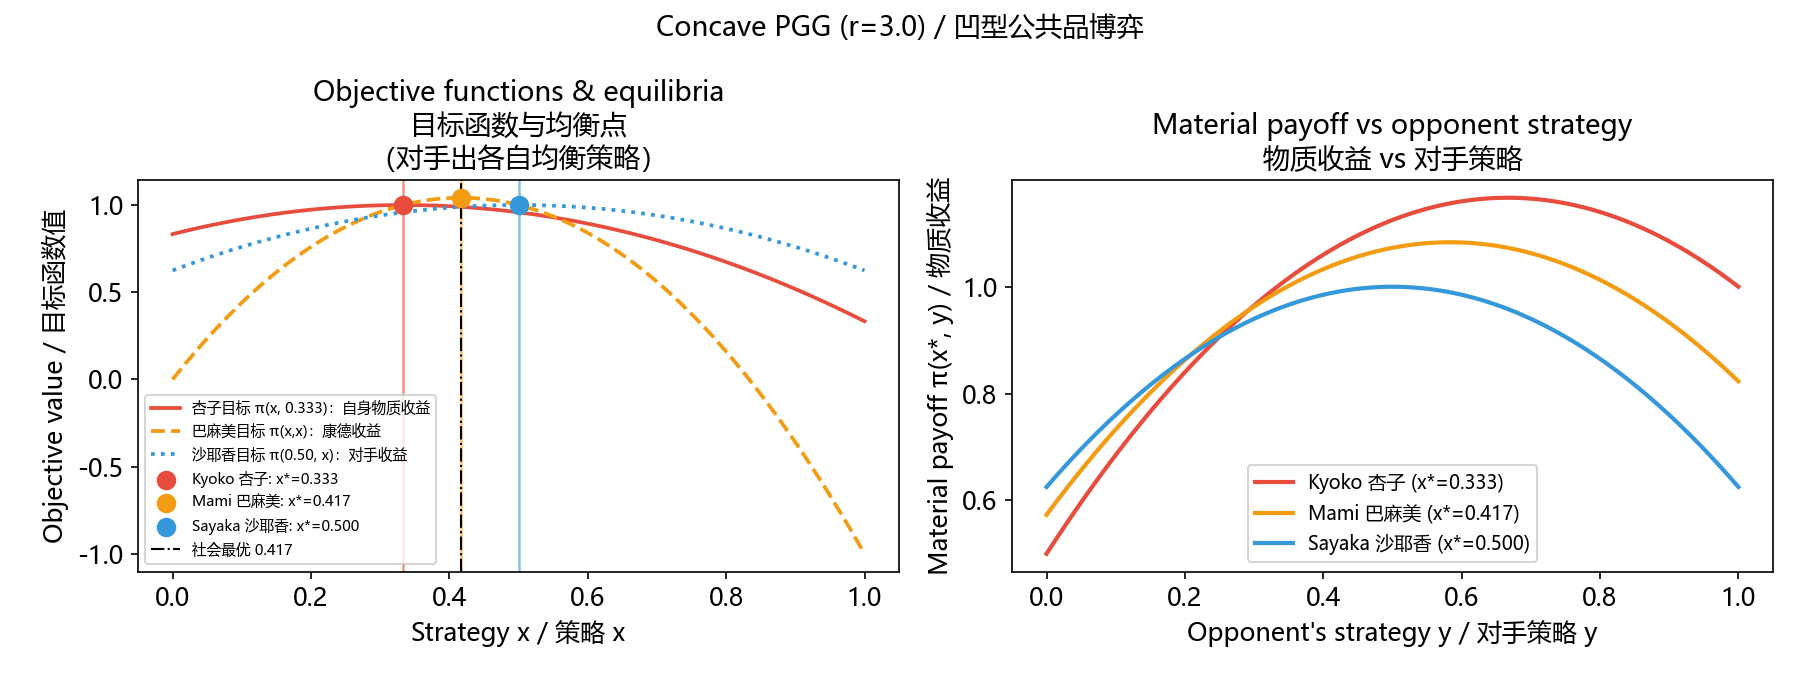
\includegraphics[width=\textwidth]{Code/madoka_strategies.png}
    \caption{左：三种类型的目标函数及均衡策略（竖线）。红实线为杏子的目标函数 $\pi(x,\, x_K^*)$（对手固定出 $x_K^*=1/3$）；橙虚线为麻美的康德目标 $\pi(x,x)$；蓝点线为沙耶香的利他目标 $\pi(x_S^*,\, x)$（对手固定出 $x_S^*=1/2$）。三条线的峰值均与各自均衡竖线对齐：每种类型在对手出相同类型均衡策略时，其目标函数恰在 $x^*$ 处取得最大值。右：固定各自均衡策略 $x^*$，物质收益随对手策略 $y$ 的变化。麻美在大多数匹配情境下的物质收益最高。}
    \label{fig:strategies}
\end{figure}

\subsection{同类匹配与适应度}

借鉴 \citet{AlgerWeibull2013} 的框架，引入\textbf{同类匹配指数} $\sigma \in [0,1]$：每次互动中，个体以概率 $\sigma$ 与同类型对手相遇，以概率 $1-\sigma$ 与整体种群随机匹配。类型 $i$ 的平均适应度为：
\begin{equation}
    f_i = \sigma \cdot \pi(x_i^*, x_i^*) + (1-\sigma) \sum_j s_j \cdot \pi(x_i^*, x_j^*),
    \label{eq:fitness}
\end{equation}
其中 $s_j$ 为类型 $j$ 在种群中的份额，$x_i^*$ 为类型 $i$ 的均衡策略（固定不变）。

在《小圆》的世界观中，$\sigma$ 对应魔法少女之间\textbf{社群紧密程度}的抽象度量。$\sigma \approx 0$ 描述的是丘比体系下魔法少女各自为战的典型状态：分散在不同地区、互不相识、与随机对手相遇——这正是 Incubator 物种所偏好的运行模式，可互换的个体在情感能量采集上效率最高，不需要形成任何共同体。$\sigma$ 较高则描述魔法少女在\textbf{紧密队伍}中协同作战的情形，同类相遇频率显著升高。因此 $\sigma$ 不仅是一个数学参数，更是对旧系统是否允许"魔法少女队伍"存在的度量：若旧系统能将 $\sigma$ 压低，则自利行为将永远占优；而高 $\sigma$ 的共同体，则构成对丘比式聚合效用最大化的内生抵抗。

\textbf{适应度}（fitness）$f_i$ 是类型 $i$ 在当前种群环境下获得的\textbf{期望物质收益}：以概率 $\sigma$ 遇到同类并获得收益 $\pi(x_i^*, x_i^*)$，以概率 $1-\sigma$ 随机遇到全体种群并获得加权平均收益。在进化博弈论框架中，适应度扮演"生存竞争力"的角色——适应度越高，意味着该类型的魔法少女平均而言获得更多资源（战斗力、灵魂宝石纯净度等的抽象代理），从而在复制动态中扩张份额。注意适应度衡量的是\textbf{物质收益}（$\pi$），而非各类型自身最大化的效用函数——杏子、麻美、沙耶香的效用函数各不相同，但进化选择仅作用于她们实际获得的物质收益。

\subsection{种群动态：丘比机制与复制动态}

魔法少女的世界中，丘比——准确来说是丘比所属的 Incubator 物种，其成员可互换、无情感、被消灭后立即由另一个替代——不断招募新的少女签订契约（进入种群），同时战斗与绝望导致魔法少女持续死亡（退出种群）。我们将此建模为\textbf{恒定总数的种群替换过程}：

\begin{itemize}
    \item 每期死亡数量等于进入数量（种群总数恒定）；
    \item 新进入者按\textbf{当前种群构成比例}抽取，即丘比的招募并无类型偏好；
    \item 死亡概率正比于\textbf{适应度的相对劣势}。
\end{itemize}

原作在这一机制上有一个值得注意的细节：魔法少女击败魔女后获得的\textbf{悲叹之种}（Grief Seed），本质上是前代魔法少女的灵魂宝石在完全绝望后凝结而成——净化自己的灵魂宝石，意味着消耗前辈的痛苦结晶。这意味着博弈中的"公共品"本身来自上一轮玩家的牺牲，系统的资源循环是自我封闭的。模型将此抽象为适应度高的类型扩张、低的类型收缩，保留了这一循环的核心逻辑而略去了其黑暗的叙事细节。

这一机制可以用三步逻辑链来理解：\textbf{适应度}反映各类型的相对生存能力 $\to$ 适应度差异决定每期的\textbf{种群替换比例}（高适应度类型更多留存，低适应度类型更多退出）$\to$ 在连续近似下，这一替换过程收敛为\textbf{复制动态方程}。

在连续近似下，上述过程等价于\textbf{标准复制动态}：
\begin{equation}
    s_i(t+1) = s_i(t) + s_i(t)\,\bigl(f_i(t) - \bar{f}(t)\bigr),
    \quad \bar{f}(t) = \sum_j s_j(t)\,f_j(t).
\end{equation}
适应度高于种群均值的类型份额增加，低于均值的类型份额减少，总份额始终归一。

模拟参数：$N = 800$ 代，初始份额均等（$s_K = s_M = s_S = 1/3$），$\sigma$ 取 $\{0.0,\, 0.25,\, 0.40,\, 0.80\}$。

%-----------------------------------------------------------------------
\section{结果}
%-----------------------------------------------------------------------

\subsection{适应度结构}

在深入讨论动态结果之前，先从适应度结构理解三者的进化命运（图~\ref{fig:fitness} 左）。

\begin{figure}[H]
    \centering
    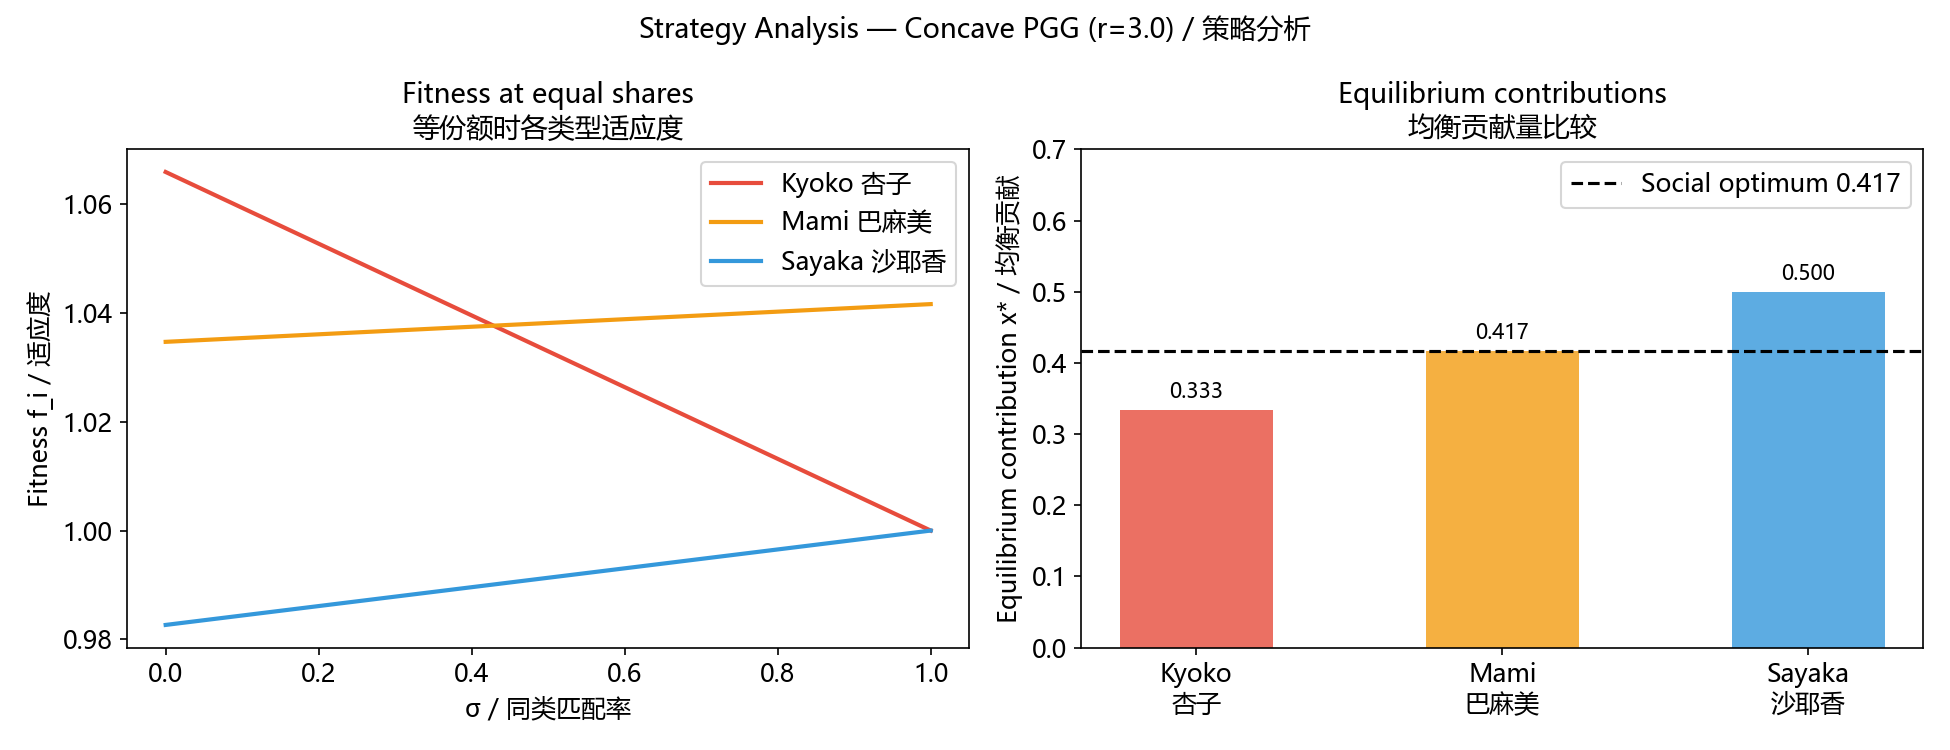
\includegraphics[width=\textwidth]{Code/madoka_fitness.png}
    \caption{左：在等份额种群（$s_K = s_M = s_S = 1/3$）下，三种类型的适应度随同类匹配率 $\sigma$ 的变化。右：三者的均衡贡献量对比，虚线为社会最优。}
    \label{fig:fitness}
\end{figure}

图~\ref{fig:fitness} 左图揭示了一个关键结构：

\begin{itemize}
    \item \textbf{杏子（红线）}：$\sigma=0$ 时适应度最高（$f_K \approx 1.067$），随 $\sigma$ 增大单调下降。原因在于，无差别随机匹配使搭便车策略最为有利；而同类匹配增加则意味着她更多地对上同样搭便车的杏子，此时双方的低贡献导致公共品不足，适应度下降。
    \item \textbf{麻美（橙线）}：适应度随 $\sigma$ 增大单调上升。同类匹配使她更多遇到另一个麻美，双方均出社会最优贡献，产生最大公共品，适应度最高。
    \item \textbf{沙耶香（蓝线）}：在\textbf{任意} $\sigma$ 下适应度均低于麻美，且低于杏子（在低 $\sigma$）或与杏子相当（在高 $\sigma$）。核心原因：$x_S^* = 0.5 > x_M^* = 0.417 = x_{\text{social}}^*$，沙耶香的过度贡献超过了凹型博弈中的边际社会收益，相当于她为他人支付了超过其实际价值的代价。她的利他不是"精准的善意"，而是"失控的慷慨"。
\end{itemize}

这一适应度结构直接预告了动态结果：沙耶香将在所有情境下被淘汰，杏子与麻美的胜负则取决于 $\sigma$。

\subsection{种群动态演化}

图~\ref{fig:population} 展示了四个 $\sigma$ 值下三种类型的份额随时间演化。

\begin{figure}[H]
    \centering
    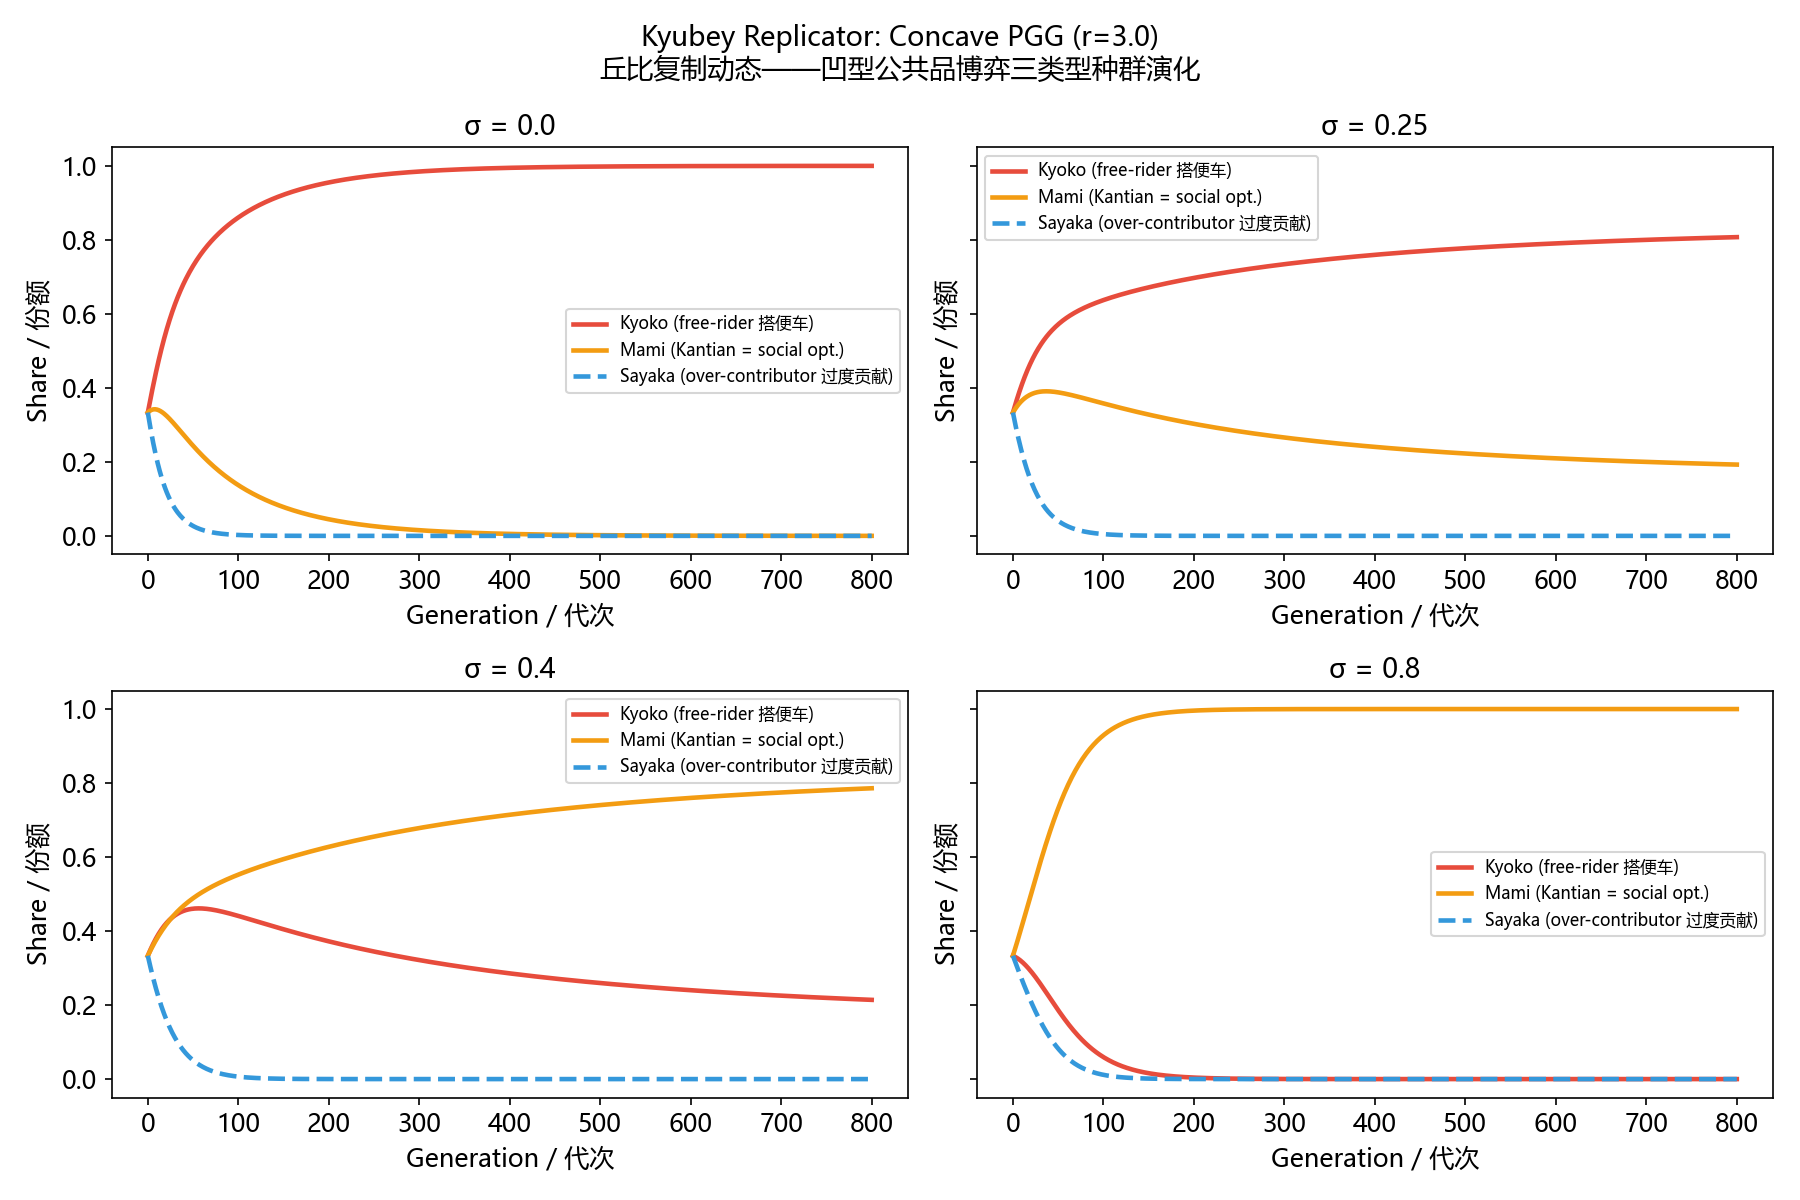
\includegraphics[width=\textwidth]{Code/madoka_population.png}
    \caption{复制动态下三种类型的份额演化（800 代）。初始均等分布 $s_K = s_M = s_S = 1/3$。四个子图分别对应 $\sigma \in \{0.0, 0.25, 0.40, 0.80\}$。}
    \label{fig:population}
\end{figure}

四个情形的结果如下：

\paragraph{$\sigma = 0.0$（完全随机匹配）} 杏子迅速主导种群，约 200 代内达到 100\% 份额。麻美和沙耶香均被淘汰。搭便车策略在陌生人匹配中无往不利——这正是标准经济学中"理性人"预测的世界。

\paragraph{$\sigma = 0.25$（低同类匹配）} 杏子仍然主导，最终份额约 63\%，麻美占 37\%，沙耶香归零。与 $\sigma=0$ 相比，麻美因偶尔遇到同类而获得一定份额，但仍输给杏子。注意：沙耶香的消失速度在此情形下实际上慢于 $\sigma=0$，因为同类匹配稍微缓解了她的适应度劣势（她与另一个沙耶香相遇时双方物质收益相等）。

\paragraph{$\sigma = 0.40$（过渡区）} 最终形成麻美（约 79\%）与杏子（约 21\%）共存的\textbf{内点均衡}，沙耶香归零。过渡过程明显：初期杏子因搭便车仍有适应度优势，维持较高份额约 100 代；随后麻美积累优势后反超，最终稳定于约 79\%。$\sigma = 0.40$ 已超过相变临界点，麻美首次获得多数份额，但两者仍共存——这是与 $\sigma = 0.80$ 时角点主导的根本区别。

\paragraph{$\sigma = 0.80$（高同类匹配）} 麻美快速主导，约 150 代内达到 100\% 份额。高同类匹配使麻美的康德策略极大受益——她几乎总是与另一个麻美相遇，产生最优公共品。杏子的搭便车优势完全丧失：即便遇到陌生人，种群中绝大多数都是麻美，低贡献策略变得得不偿失。

\subsection{相图：匹配率与最终格局}

图~\ref{fig:phase} 展示了在 $\sigma$ 从 0 到 1 连续变化时，稳态种群构成的全貌。

\begin{figure}[H]
    \centering
    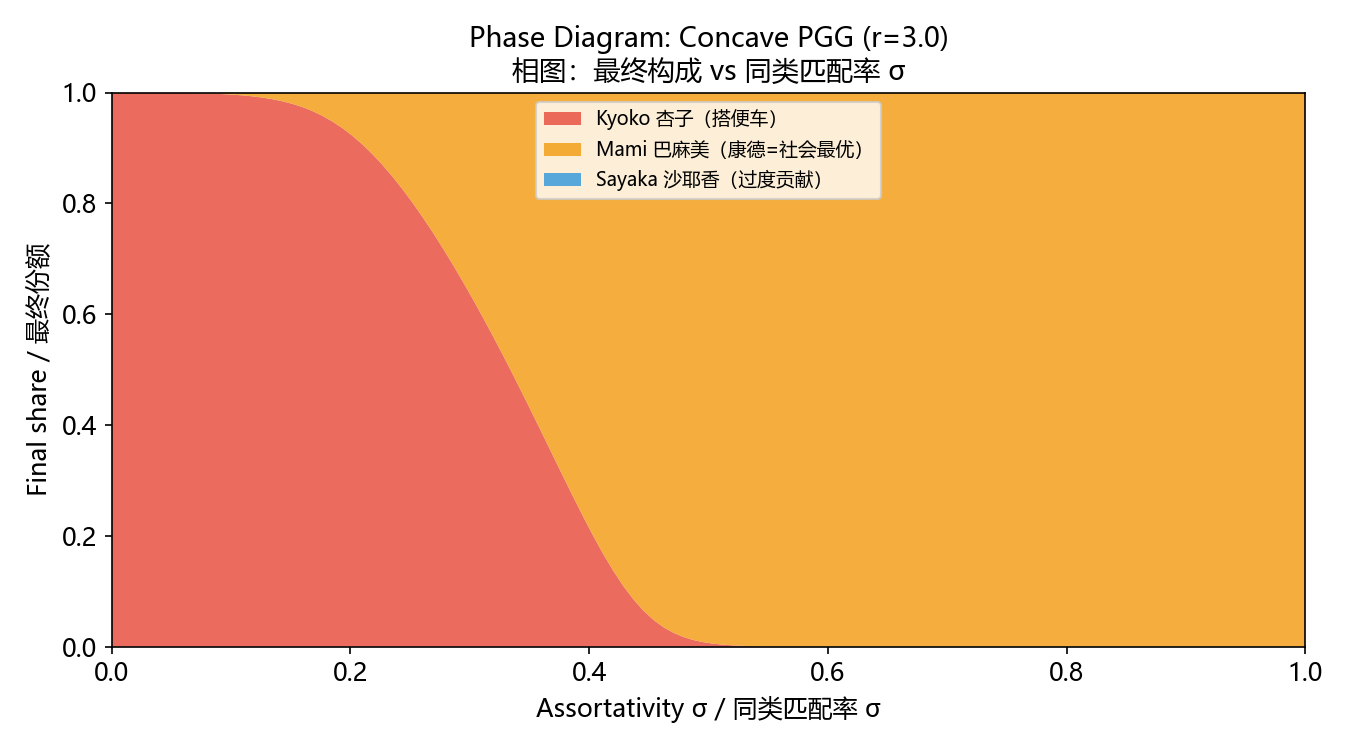
\includegraphics[width=0.85\textwidth]{Code/madoka_phase.png}
    \caption{稳态种群构成随同类匹配率 $\sigma$ 的变化（堆叠面积图）。蓝色区域（沙耶香）在全程均为零，故不可见。}
    \label{fig:phase}
\end{figure}

相图揭示了清晰的\textbf{相变结构}：
\begin{itemize}
\item $\sigma \lesssim 0.25$：杏子（Kyoko）几乎完全主导，麻美（Mami）份额接近于零。

\item $0.25 \lesssim \sigma \lesssim 0.50$：过渡区。随着同类匹配率 $\sigma$ 增大，麻美的份额逐渐上升，而杏子的份额持续下降。

\item $\sigma \approx 0.35$：临界附近，两种类型的份额大致相当。

\item $\sigma \gtrsim 0.50$：麻美成为几乎唯一稳定类型，杏子的份额迅速趋近于零。

\item 沙耶香（蓝色）在整个 $\sigma\in[0,1]$ 范围内份额恒为零，完全淘汰。
\end{itemize}

相变并非突变，而是 S 形过渡：在临界点附近，适应度差异最小，过渡最慢。这与图~\ref{fig:population} 中 $\sigma=0.40$ 情形下麻美反超杏子的曲折过程一致。

\subsection{单纯形相图：轨迹结构}

图~\ref{fig:simplex} 以三维单纯形相图的形式展示了从不同初始条件出发的种群轨迹，三角形的三个顶点分别代表三种类型全部主导的极端情形。

\begin{figure}[H]
    \centering
    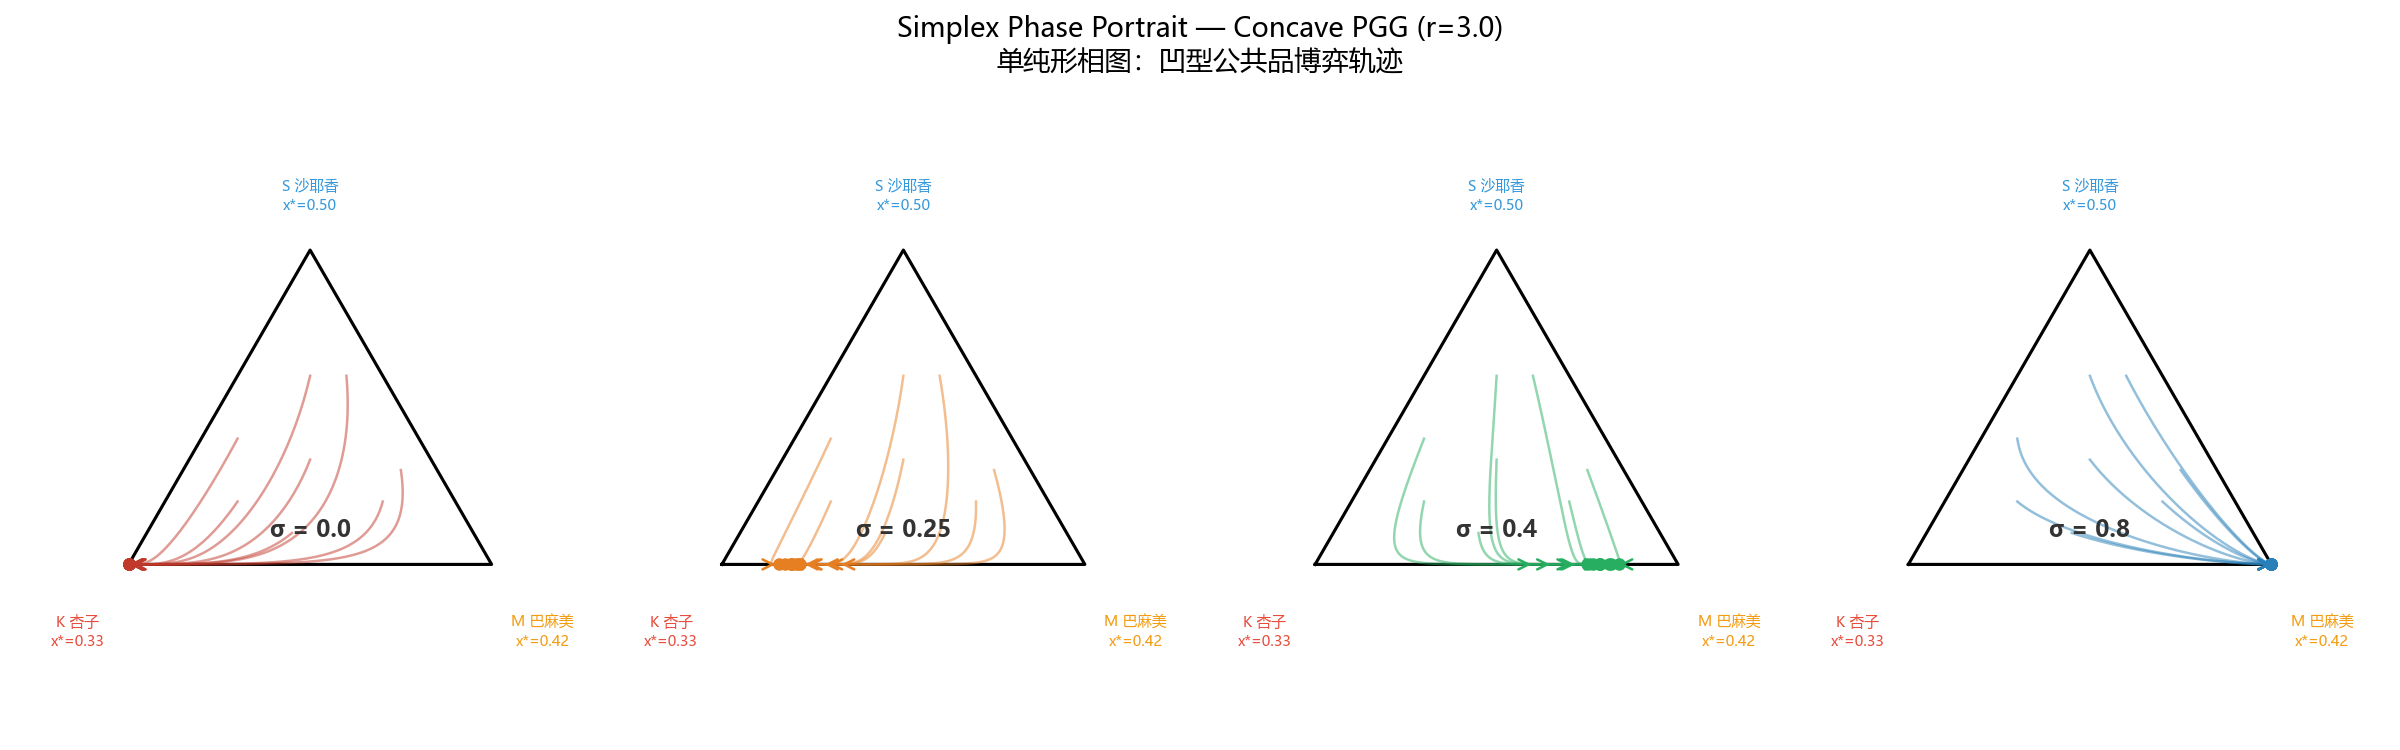
\includegraphics[width=\textwidth]{Code/madoka_simplex.png}
    \caption{单纯形相图。三角形顶点分别为 K（杏子主导）、M（麻美主导）、S（沙耶香主导）。各条轨迹从不同初始分布出发，箭头标示演化方向，终点为吸引子。}
    \label{fig:simplex}
\end{figure}

单纯形相图揭示了系统的\textbf{全局动态结构}：

\begin{itemize}
    \item \textbf{$\sigma = 0.0$}：所有轨迹均流向 K 顶点（杏子），无论初始构成如何。K 是全局吸引子。注意轨迹首先沿底边（K-M 轴）运动，S 份额迅速消失，然后杏子主导麻美。

    \item \textbf{$\sigma = 0.25$}：吸引子在 K-M 轴上的内点（杏子约 63\%，麻美约 37\%），不再是纯角点。S 份额同样迅速归零。轨迹先垂直向底边收缩，再沿底边向 K-M 混合均衡收敛。

    \item \textbf{$\sigma = 0.40$}：吸引子为 K-M 轴上的\textbf{内点}（麻美约 79\%，杏子约 21\%），不再是纯角点。轨迹经历明显的"迁回"：部分初始条件下种群先向 K 方向移动，再折回趋向该内点均衡。这体现了临界点附近的动态复杂性。

    \item \textbf{$\sigma = 0.80$}：所有轨迹径直流向 M 顶点，收敛极快。麻美是唯一吸引子，且吸引盆覆盖整个单纯形。
\end{itemize}

值得注意的是，\textbf{S 顶点（沙耶香主导）从未成为吸引子}，也没有任何轨迹趋向该方向——沙耶香的纯利他偏好在进化上是完全不稳定的，无论初始构成或匹配环境如何。

%-----------------------------------------------------------------------
\section{讨论}
%-----------------------------------------------------------------------

\subsection{沙耶香悲剧的博弈论诠释}

沙耶香在原作中因\textbf{期望与现实的落差}走向绝望：她以为无私的牺牲会带来美好结果，却发现自己的善意换来了冷漠。本模型提供了一个结构性解释：\textbf{纯利他偏好在进化博弈中是不稳定的}，不是因为"善意本身有错"，而是因为她的策略（$x_S^* = 0.5$）系统性地超过了帕累托最优水平（$x_M^* = 0.417$），无论面对什么类型的对手，她的物质收益都低于麻美。

用模型的语言：沙耶香将对手的效用函数内化为自己的效用函数，但对手的最优并非全局最优。在一个回报递减的世界里，过度贡献既伤害自己，也不能帮助他人超过麻美式的精准贡献。

从伦理叙事的层面看，$u_S = \pi(y,x)$ 这一形式化背后隐藏着沙耶香对\textbf{动机纯洁性}的极端要求：她必须相信自己的行为完全无私，才能维持伦理道路的正当性。一旦她承认救恭介中夹杂着个人的爱慕与执念，承认自己也会嫉妒与受伤，整个自我叙事便会崩溃。完全将对手效用内化为自身效用，在数学上等价于拒绝承认任何自我利益的存在；而这种拒绝正是她策略性过度贡献的伦理根源。因此，沙耶香的悲剧不仅是"贡献量超过社会最优"的效率问题，更是一种\textbf{不允许人性复杂性存在的伦理纯洁}在结构性压力下必然走向自我瓦解——旧系统的残酷之处，恰在于它精准地击穿了这种纯洁所赖以成立的前提。

原作在叙事结构上将这一悲剧编码进了沙耶香的魔女形态：她化身的魔女 Oktavia von Seckendorff 是一只困在充满音乐厅与提琴声的结界里的巨大装甲人鱼，其原型直接来自安徒生《海的女儿》——一个为了爱人牺牲了自己的声音（表达自身感受的能力），最终走向消逝的形象。从某种意义上讲，人鱼公主失去的"声音"，正是说出"我也有自己的需求"的能力；而沙耶香的效用函数 $u_S = \pi(y,x)$ 所做的，正是在数学上抹去了这个声音。她的魔女形态因此成为这一偏好结构的终极隐喻：彻底放弃自己的效用函数，最终被困在一个永远只能回响他人音乐的结界里。

\subsection{麻美的“胜利”：康德即效率}

麻美的胜利有一个深刻的内在原因：\textbf{在凹型公共品博弈中，康德道德律令与社会最优解重合}。当她问"若所有魔法少女都如此行动，结果如何？"时，她恰好找到了使总社会福利最大的策略。这不是巧合，而是博弈结构的必然：凹型博弈的社会最优正是由"全体均出此贡献量"所定义的。

因此，高同类匹配环境（紧密社群、魔法少女队伍内部等）天然有利于麻美式的道德：同类相遇时，双方的康德策略恰好形成最优均衡，适应度最高。

然而，麻美的稳定有一个结构性前提：她所履行的"保护"必须真正对应"保护"。原作中，在某条时间线里，当麻美得知魔法少女最终都会变成魔女时，她立刻崩溃，甚至试图亲手杀死同伴——以一种扭曲的"保护"逻辑阻止她们走向更坏的结局。这恰好印证了模型的结构预测：麻美的康德策略在高 $\sigma$ 环境中具有最强适应性，但这一适应性以"职责与结果之间的对应关系成立"为前提。一旦博弈结构本身被颠覆，她的伦理大厦便会与基础一同坍塌。

值得注意的是，麻美的稳定并非来自对某种道德纯洁的坚守，而是一种\textbf{务实的伦理底色}：她无需相信自己动机的绝对高尚，也无需用"善意必有善果"的朴素信念撑起行动——她只需要问"若所有魔法少女都如此行动，结果会怎样"，便自然找到了社会最优解。$u_M = \pi(x,x)$ 的形式化是一种关于\textbf{行动结构的理性原则}，而非关于动机纯粹性的道德说教；正因如此，它能够承受动机的复杂性而不崩溃，与沙耶香对纯洁性的执念形成了对比。麻美从未将对手的效用内化为自身效用，因而也从未暴露在过度贡献的崩溃模式之下。

\subsection{杏子的理性：世界设定的问题}

杏子并非失败——她的策略在低匹配率环境中是进化上最优的。她的“失败”发生在高 $\sigma$ 的世界。这提示我们：\textbf{道德偏好的进化稳定性不取决于偏好本身的"好坏"，而取决于社会匹配结构}。在一个陌生人频繁互动的分散世界（低 $\sigma$）里，纯自利理性是均衡的；在一个紧密共同体（高 $\sigma$）里，康德道德是均衡的。

Alger \& Weibull（2013）的主定理正是如此断言：进化稳定类型为 homo moralis，其康德系数恰等于同类匹配指数 $\kappa^* = \sigma$。本文的三类型模型是该定理在离散偏好类型空间上的一个例示。

需要指出的是，本模型将杏子的 $u_K = \pi(x,y)$ 视为外生给定的偏好类型。但原作的叙事提示了一种更深的解读：她的自利理性并非天生禀赋，而是一种伦理幻灭后的哲学残留。她最初许愿是为了让父亲的布道被更多人听见，背后隐含着"善意终有善果"的朴素期待；然而家破人亡的结局彻底击碎了这一信念，迫使她退到"先保全自己"的生存主义立场。因此，模型中的纯自利类型，在叙事层面更接近\textbf{一种经历了结构性背叛之后主动构建的生存策略}，而非先验给定的人性底色。

原作中，打破这一生存主义立场的正是沙耶香——一个走上了杏子曾经走过道路的人。杏子在沙耶香身上认出了过去的自己：同样为他人许愿，同样遭遇背叛，同样在理想破灭后滑向绝望。

这一识别改变了博弈的结构。对杏子而言，沙耶香不再只是一个博弈中的对手，而是一个与自己共享起点的“镜像”。然而，在当前的世界中，这一类型已经无法稳定存在：沙耶香的转化几乎不可逆转。

因此，杏子的选择并不是策略上的重新计算，而更接近于一种退出博弈的行为。通过与沙耶香同归于尽，她拒绝继续参与一个已经失去意义的博弈结构。

在叙事层面，这一行为表现为牺牲；而在模型语言中，它可以被理解为当个体意识到某一偏好类型在当前环境中已无进化空间时，对该博弈结构的终止性回应。

这一观察也指向一个超出本文静态框架的问题：如果偏好类型本身能够在长期制度或环境压力下发生内生演化，那么魔法少女世界中纯自利理性的盛行，或许并非单纯的个体选择，而可能反映了丘比（Incubator）所主导的旧系统对行为类型的长期筛选。在一个低同类匹配率的环境中，自利型策略更容易在进化上存活，从而逐渐成为主导行为模式。

%-----------------------------------------------------------------------
\section{结论}
%-----------------------------------------------------------------------

本文以《魔法少女小圆》中的三位角色为载体，构建了一个三类型凹型公共品进化博弈模型。主要结论如下：

\begin{enumerate}
    \item \textbf{纯利他偏好（沙耶香）在进化上始终不稳定。} 在任何匹配环境下，沙耶香的过度贡献使她的适应度系统性低于麻美，最终被淘汰。这为原作中沙耶香的悲剧提供了一个结构性的博弈论诠释。

    \item \textbf{杏子（自利）与麻美（康德）的“胜负”由匹配结构决定。} 低同类匹配率（$\sigma < 0.35$）有利于搭便车的杏子；高匹配率（$\sigma > 0.35$）有利于实现社会最优的麻美。临界点约在 $\sigma \approx 0.35$。

    \item \textbf{在凹型公共品博弈中，康德道德律令等价于社会效率，而利他主义并不等同于效率。} 麻美的”胜利”不是”道德战胜了自私”，而是”社会最优偏好战胜了偏离均衡的偏好”——包括过度自利（杏子）和过度利他（沙耶香）。这揭示了一个反直觉的对称性：在回报递减的博弈结构中，贡献过少（搭便车）与贡献过多（过度利他）是\textbf{两种对称的偏离}，沙耶香的策略与杏子的策略都远离社会最优，只是方向相反。”为他人着想”并不自动等于”对社会有益”——关键在于贡献量是否恰好处于社会最优水平。

    \item \textbf{丘比的招募机制等价于标准复制动态。} 恒定种群、按当前构成进入的设定使进化选择完全由适应度差异驱动，与标准进化博弈论吻合。
\end{enumerate}

最后，以一句话总结本文的核心洞见：\textbf{在一个回报递减的世界里，进化不奖励最无私的人，而奖励恰到好处的人。}

\bibliographystyle{plainnat}
\bibliography{references}
 
\end{document}
